\documentclass[../mathNotesPreamble]{subfiles}
\begin{document}
    \section{JIT 5.3: Special angles $\parens{\dfrac{\pi}{4}, \dfrac{\pi}{6}, \dfrac{\pi}{3}}$}
    
    \begin{minipage}{0.5\linewidth}
      \begin{tikzpicture}
        \draw (0,0) -- (8,0) -- (4,6.928) -- cycle;
        \draw[dashed] (4,0) -- (4,6.928);
        \draw (3.65,0) -- (3.65,0.35) -- (4,0.35);
        \node at (1.5,3.75) {1};
        \node at (6.5,3.75) {1};
        \node at (4,-0.5) {1};
      \end{tikzpicture}
    \end{minipage}%
    \begin{minipage}{0.5\linewidth}
      \begin{center}
        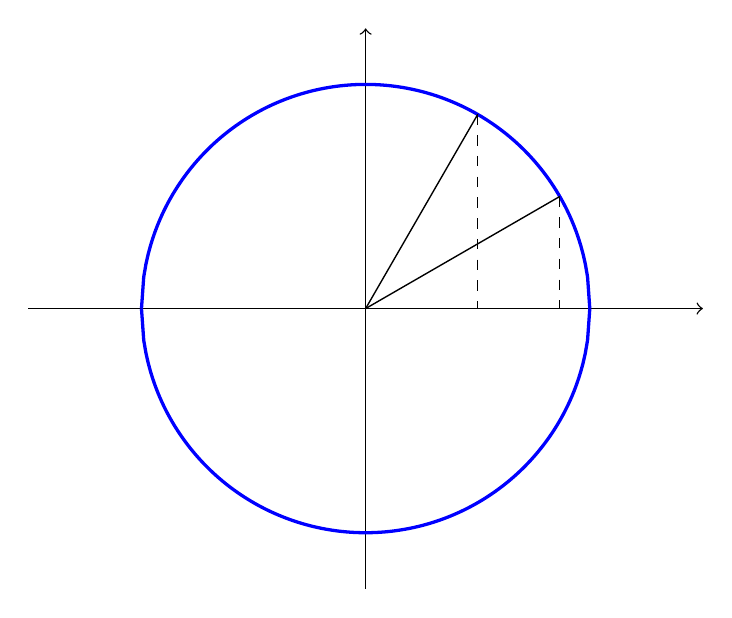
\begin{tikzpicture}[scale=1.25]
          \begin{axis}[
            axis lines=center,
            axis equal, 
            axis line style={->},
            ymin=-1.25, ymax=1.25,
            xmajorticks=false,
            ymajorticks=false,
            every axis plot/.append style={line width=0.95pt},
            ]
              \addplot[domain=-1:1, blue, samples=201] {sqrt(1-x^2)};
              \addplot[domain=-1:1, blue, samples=201] {-sqrt(1-x^2)};
              \draw (axis cs: 0,0) -- (axis cs: 0.5,0.866);
              \draw (axis cs: 0,0) -- (axis cs: 0.866,0.5);
              \draw[dashed] (axis cs: 0.866,0.5) -- (axis cs: 0.866,0);
              \draw[dashed] (axis cs: 0.5,0.866) -- (axis cs: 0.5,0);
          \end{axis}
        \end{tikzpicture}
      \end{center}
    \end{minipage}
    
    \vspace*{\stretch{1}}
    \begin{minipage}{0.475\linewidth}
      \begin{tikzpicture}[scale=0.85]
        \draw (0,0) -- (8,0) -- (8,8) -- cycle;
        \draw (7.65,0) -- (7.65,0.35) -- (8,0.35);
        \node at (4,4.5) {1};
        \node at (8.5,4) {s};
        \node at (4,-0.5) {s};
      \end{tikzpicture}
    \end{minipage}%
    \begin{minipage}{0.5\linewidth}
      \begin{center}
        \begin{tikzpicture}[scale=1.25]
          \begin{axis}[
            axis lines=center,
            axis equal, 
            axis line style={->},
            ymin=-1.25, ymax=1.25,
            xmajorticks=false,
            ymajorticks=false,
            every axis plot/.append style={line width=0.95pt},
            ]
              \addplot[domain=-1:1, blue, samples=201] {sqrt(1-x^2)};
              \addplot[domain=-1:1, blue, samples=201] {-sqrt(1-x^2)};
              \draw (axis cs: 0,0) -- (axis cs: 0.707,0.707);
              \draw[dashed] (axis cs: 0.707,0.707) -- (axis cs: 0.707,0);
          \end{axis}
        \end{tikzpicture}
      \end{center}
    \end{minipage}
    \pagebreak
    \vspace*{\stretch{0.75}}
    \begin{center}
      \newcommand{\aRad}{0.575}
      \newcommand{\rRad}{0.875}
      \newcommand{\cRad}{1.2}
      \newcommand{\lCol}{gray!90}
      \begin{tikzpicture}[scale=7.0]
        \draw[line width=1pt] (0,0) circle(1);
        \foreach \x in {0,30,...,360} {
        \draw[\lCol] (0cm,0cm) -- (\x:1);
        }
        
        \foreach \x in {45,135,225,315} {
          \draw[\lCol] (0cm,0cm) -- (\x:1);
          }
        \ifprintanswers\foreach \x/\xtext in {
          30/\dfrac{\pi}{6},
          45/\dfrac{\pi}{4},
          60/\dfrac{\pi}{3}}
          \draw (\x:\rRad) node[fill=white] {$\xtext$};
      \foreach \x/\xtext/\y in {
        30/\frac{\sqrt{3}}{2}/\frac{1}{2},
        45/\frac{\sqrt{2}}{2}/\frac{\sqrt{2}}{2},
        60/\frac{1}{2}/\frac{\sqrt{3}}{2}}
          \draw (\x:\cRad) node {$\left(\xtext,\y\right)$};
      \draw (-\cRad,0cm) node{$(-1,0)$}
            (\cRad,0cm)  node{$(1,0)$}
            (0cm,-\cRad) node{$(0,-1)$}
            (0cm,\cRad)  node{$(0,1)$};\fi
      \end{tikzpicture}
    \end{center}
    \vspace*{\stretch{1}}
    
    \pagebreak
\end{document}